%%%%%%%%%%%%%%%%%%%%%%% preamble %%%%%%%%%%%%%%%%%%%%%%%%%%%
\documentclass[10pt,letterpaper]{article}
\usepackage{opex3}
%\usepackage{graphicx}
\usepackage{hyperref}
\usepackage{amssymb}
\hypersetup{colorlinks=true,
		      urlcolor=blue}
\usepackage{amsmath}      
\usepackage{bm}
\newcommand{\myeqno}[1]{Eq.~\eqref{#1}}
\DeclareMathOperator*{\argmin}{arg\,min}
%%%%%%%%%%%%%%%%%%%%%%% begin %%%%%%%%%%%%%%%%%%%%%%%%%%%%%%
%\linespread{1.25}
\begin{document}
\title{\Large{Assignment 1: Supervised learning}}
\author{\href{mailto:rohan.kekatpure@gmail.com}{Rohan D. Kekatpure}}
\address{}
\email{}

\begin{thebibliography}{9}
\bibitem{mnist} 
MNIST handwritten digit database.\\
\href{\tt http://yann.lecun.com/exdb/mnist/}{http://yann.lecun.com/exdb/mnist/}

\bibitem{ionosphere}
Ionosphere data at UCI.\\
\href{\tt https://archive.ics.uci.edu/ml/machine-learning-databases/ionosphere/ionosphere.names}{https://archive.ics.uci.edu/ml/machine-learning-databases/ionosphere/ionosphere.names}

\bibitem{kegl}
B.~Kegl and R.~Busa-Fekete
{\it Boosting products of base classifiers} \\
\href{\tt https://www.lri.fr/~kegl/research/PDFs/KeBu09.pdf}{https://www.lri.fr/~kegl/research/PDFs/KeBu09.pdf}
%\bibitem{einstein} 
%Albert Einstein. 
%\textit{Zur Elektrodynamik bewegter K{\"o}rper}. (German) 
%[\textit{On the electrodynamics of moving bodies}]. 
%Annalen der Physik, 322(10):891?921, 1905. 
\end{thebibliography}

\section{Description of the datasets}
This assignment asks us to apply five supervised learning algorithms on two datasets. The main goal of this exercise to understand the trade-offs in using these algorithms for real-world data mining and predictive modeling tasks. To accomplish this, one needs to identify non-trivial datasets rich in features and size to allow such comparative study. I have chosen the \href{http://yann.lecun.com/exdb/mnist/}{MNIST} \cite{mnist} and the \href{Its a binary classification problem allowing an easier comparative analysis of various learning algorithms.}{Ionosphere observations} \cite{ionosphere} datasets for my study. 

\subsection{What makes these datasets interesting?} 
The MNIST is a classic image recognition benchmark dataset consisting of 60000 labeled images of handwritten digits in the training set and 10000 in the testing set. Ionosphere observation dataset is 350 observations of 34 attributes with an objective to classify them into `good' `bad' observations. I believe the following factors qualify these datasets as `interesting':
%%
\subsubsection*{MNIST}
\begin{enumerate}
	\item It has been used to benchmark a number of learning algorithms in image recognition, allowing comparisions to published studies.
	\item Each training example is a $28\times28$ pixels image giving a dimensionality of 784. At this scale, dimensionality is expected to affect model performance, especially for `sampling' type of algorithms (e.g. nearest-neighbor-type algorithms). 
	\item Its a multi-class classification problem. While this makes it difficult to benchmark performance of some inherently binary classifiers, it is problem representative of the real world classification tasks we're likely to encounter. 
	\item {\color{magenta} By using this dataset I'm taking the risk of not being able to train some algorithms (boosted trees) on the full dataset on my laptop. However, I've always been curious about performance of different learning algorithms on MNIST and would like to see how far I get given my limited computational resources.}
\end{enumerate}
%%
\subsubsection*{Ionosphere}
For our studies, we include 150 observations in our training set and use the remaining 201 observations for testing. We don't know the train/test split use by the published studies, which might affect how closely we're able to reproduce these results.
\begin{enumerate}
	\item Ionosphere is a binary classification problem with 34 attributes. Its binary nature allows an easier comparative analysis of various binary classification algorithms.  
	\item Ionosphere data is relatively smaller in comparison to MNIST. Its smaller size will allow us to efficiently train our models on a laptop. We plan to use this data especially to learn more about boosted tree ensembles.  
\end{enumerate}
%%
\section{Supervised learning on the MNIST data}
\subsection{$k$ nearest neighbors (KNN)}
Given a test instance, KNN performs a (linear) lookup in the training set and returns the label of the instance closest to the test instance according to some distance metric. For $k>1$, KNN performs a majority vote between the labels. For the MNIST data, the training examples are 1 dimensional arrays with size 784 and the individual elements having integer values between 0 to 255. The Euclidean distance between two image arrays $a$ and $b$ is defined as:
\begin{equation}
	d(a,b) = \left[\sum_{i=0}^{784}(a_i - b_i)^2\right]^{1/2}
\end{equation}

Figure~\ref{knn1} shows the evolution of the error (defined as misclassification rate) for the training and the test sets as we vary the number of nearest neighbors. Two major conclusions are evident from the figure.
\begin{figure}[tbp]
	\begin{center}
	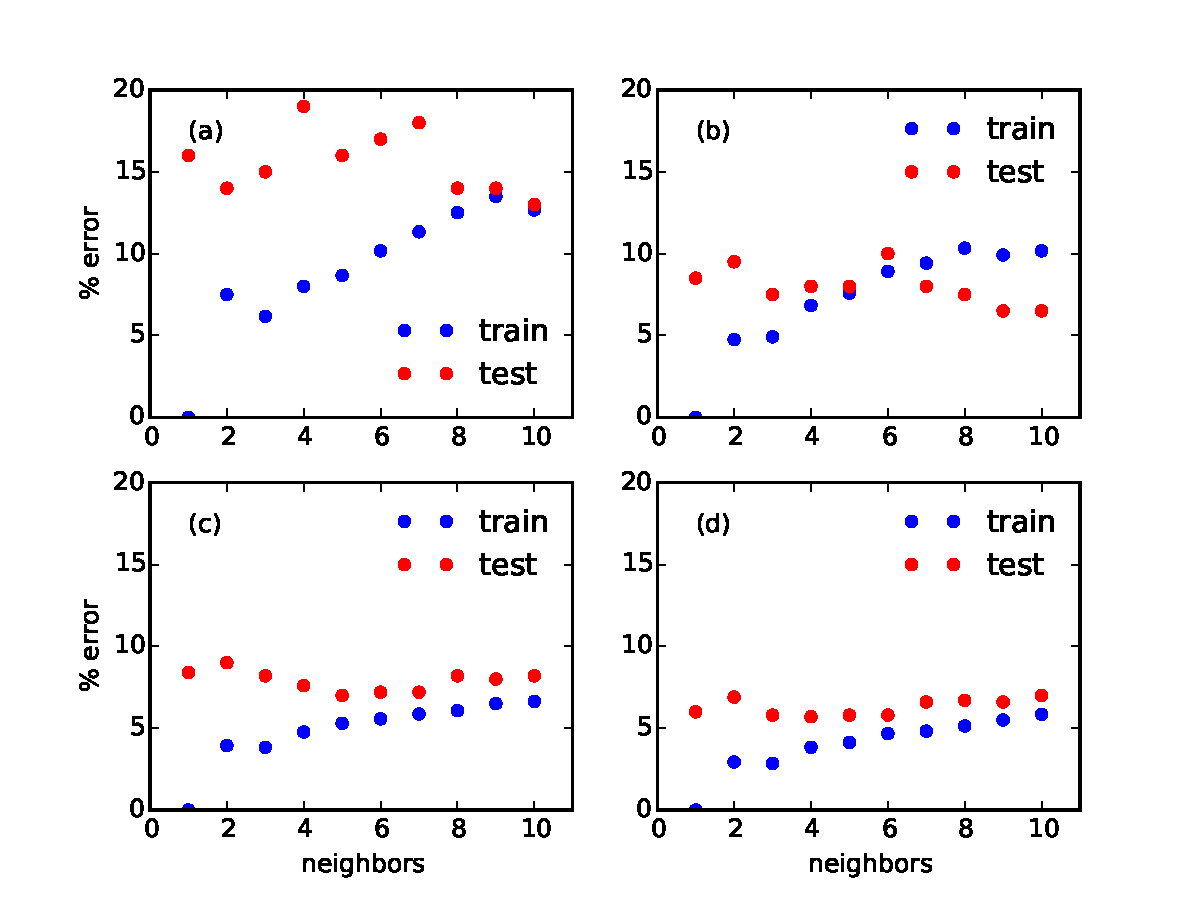
\includegraphics[width=4in]{../results/mnist/knn/error_vs_nbrs.pdf}
	\end{center}
	\caption{Error evolution of KNN algorithm with number of nearest neighbors for different sizes of the training set. The value of $N_{\text{train}}$ are as follows: (a) 600, (b) 1200, (c) 3000 and  (d) 6000. In all subfigures, test error is depicted in {\color{red} red} and training error is {\color{blue} blue}. \label{knn1}}
\end{figure}
%%
First, because of the high dimensionality of the problem, the KNN algorithm is expected to need large amounts of the data to sample any reasonable neighborhood of a given test instance. Consequently the model performs better as the dataset size is increased. The cost, however, is a linearly increasing lookup time. For a training set size of 6000, the lookup for all training examples takes over 30 minutes. Therefore all results are reported only up to a $N_{\text{train}} = 6000$ sample size. 

Second, the training and test errors show opposite variations with increasing $k$, the number of nearest neighbors. Training error {\em increases} with $k$ while the test error {\em decreases}. With a small $k$, the algorithm is averaging over a small local region around the test instance causing inclusion of more noise. In other words, with small $k$ the model is overfitting. Increasing $k$ and averages over larger sample lead to better generalization and smaller test error (Fig.~\ref{knn2}). 
%
\begin{figure}[tbp]
	\begin{center}
	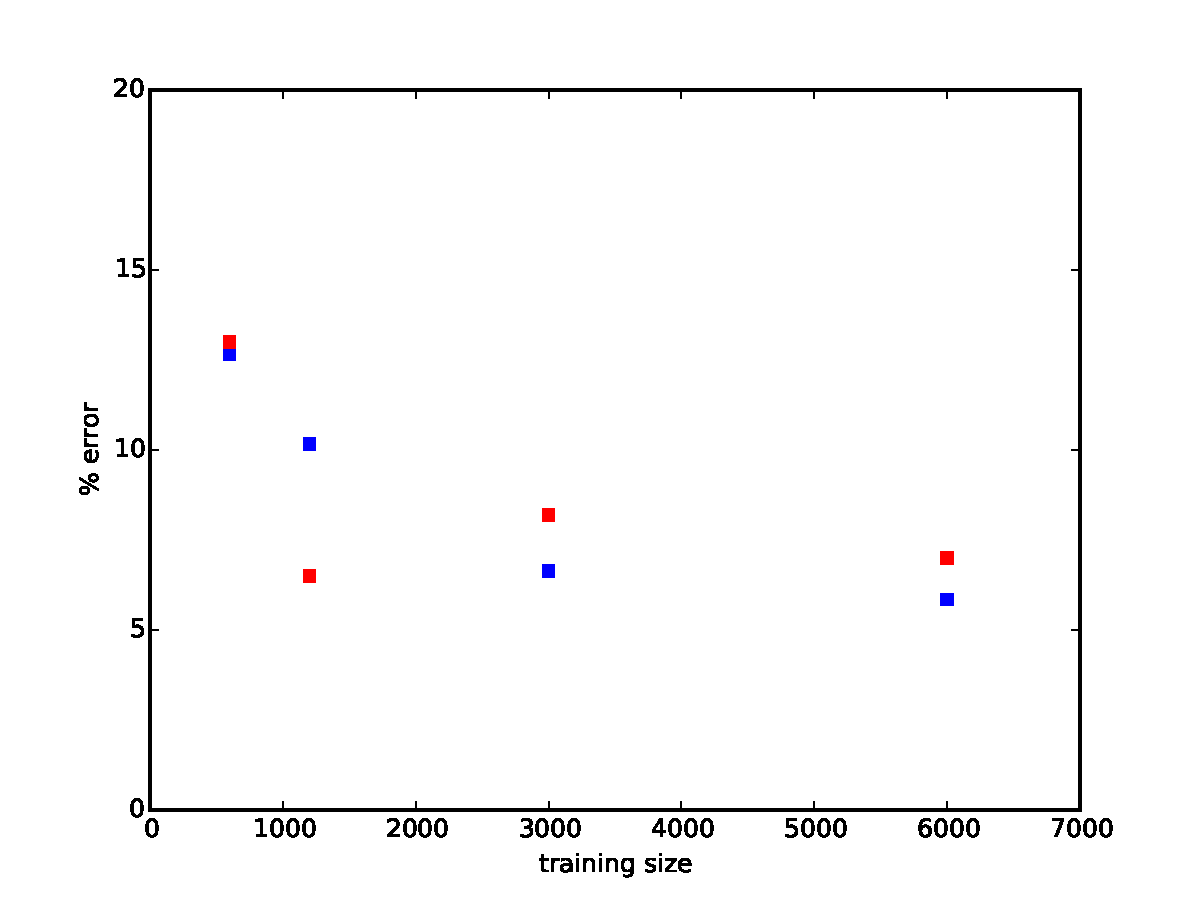
\includegraphics[width=2.5in]{../results/mnist/knn/error_vs_training_size.pdf}
	\end{center}
	\caption{Misclassification rate of the KNN algorithm with training set size \label{knn2}}
\end{figure}
%

{\bf Model improvement:} Given the simplicity of the KNN algorithm, it is remarkable that it is able to achieve a $\sim95\%$ accuracy on an image classification task with only 6000 training samples. Because of the high dimensionality of the problem, the error is expected to decrease even more with increase in the size of the training data, albeit at the cost of increased prediction time. The fundamental issue of nearest-neighbor classifiers is the curse of dimensionality. One way to improve performance of the KNN model might be to use dimensionality reduction techniques like principal component analysis (PCA) and perform the lookup in the space of reduced dimensions. 
%%
\subsection{Decision trees}
Single decision trees tend to perform well on problems with a small number of discrete attributes. The MNIST dataset, in contrast, has 784 attributes that are practically continuously spaced (0 through 255 with a spacing of 1). As such, we'd be justified in having doubts about performance of single decision trees for this dataset. 
%%
\begin{figure}[tbp]
	\begin{center}
	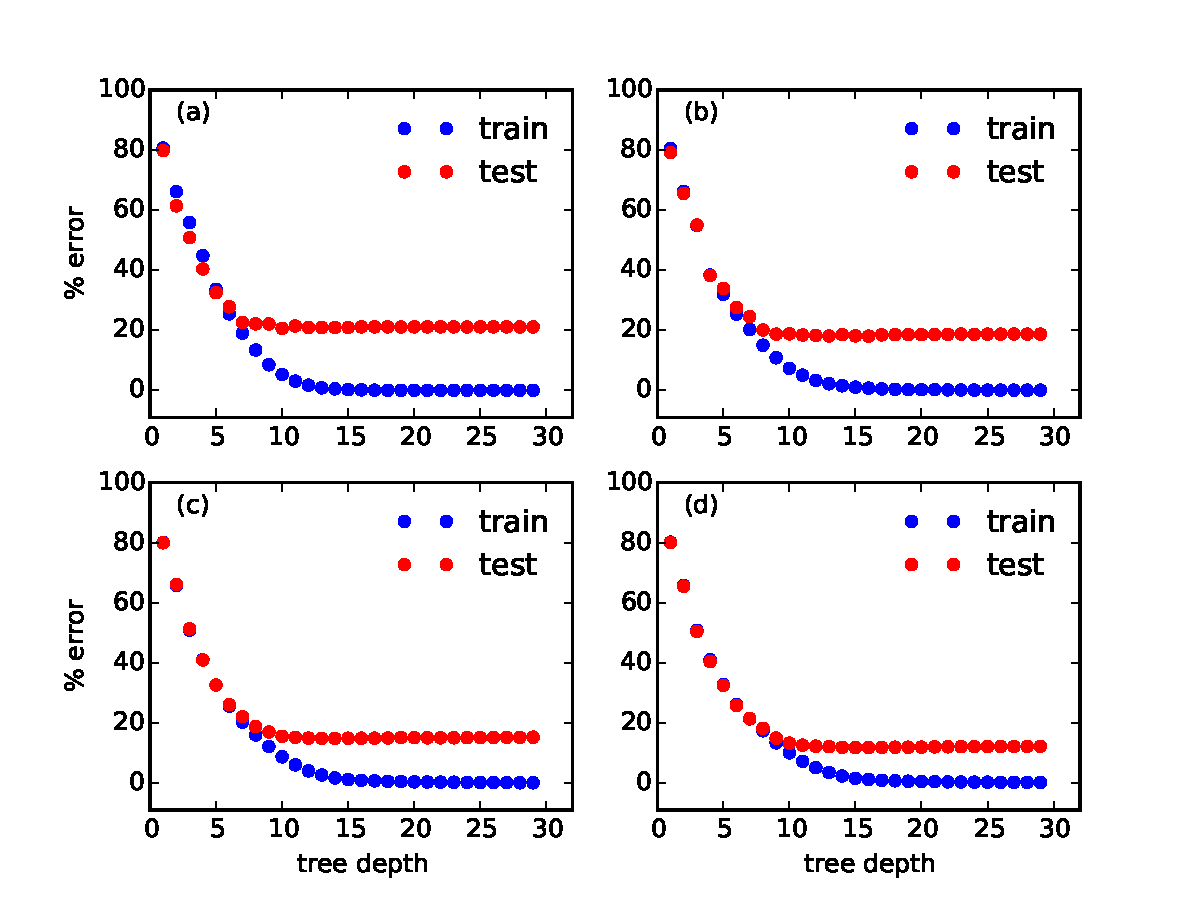
\includegraphics[width=4in]{../results/mnist/dtree/error_vs_depth.pdf}
	\end{center}
	\caption{Misclassification rate of the decision tree algorithm with depth of the tree for varying dataset sizes. The size of the training data is (a) 6000, (b) 12000, (c) 30000 and (d) 60000 training samples.\label{dtree1}}
\end{figure}
%%

We ran decision tree algorithm using the {\tt rpart} package in R. In addition to rapidly computing the trees, {\tt rpart} is also able to perform pruning using the depth of the tree ({\tt maxdepth} parameter) as well as the marginal information gain (via the {\tt complexityParameter}). To determine the optimal tree size, we first studied the error evolution as a function of the tree depth. 

Figure~\ref{dtree1} shows the variation of the training and test error with increasing tree depth. Although not visible at the scale of the figure, the test error {\em increases} for $\texttt{maxdepth}>15$, clearly signifying overfitting. The performance of the model is significantly worse compared to the KNN. The minimum error rate for 6000 samples (corresponding to Fig~\ref{knn1}(d)) is $\sim21\%$ almost four times that of KNN trained on similar volume of data. Even training the model on the full dataset of 60000 samples improves the error rate to $\sim12\%$, still double that of KNN trained on 1/10th of data. 

Next, we fixed $\texttt{maxdepth} = 15$ and studied the model performance (as measured by misclassification error) with number of nodes. For $N=6000$ training samples, there is a clear evidence of overfitting with increasing number of nodes (model complexity). For $N=60000$ training examples, the over fitting is less evident, but is numerically present. 

%%
\begin{figure}[tbp]
	\begin{center}
	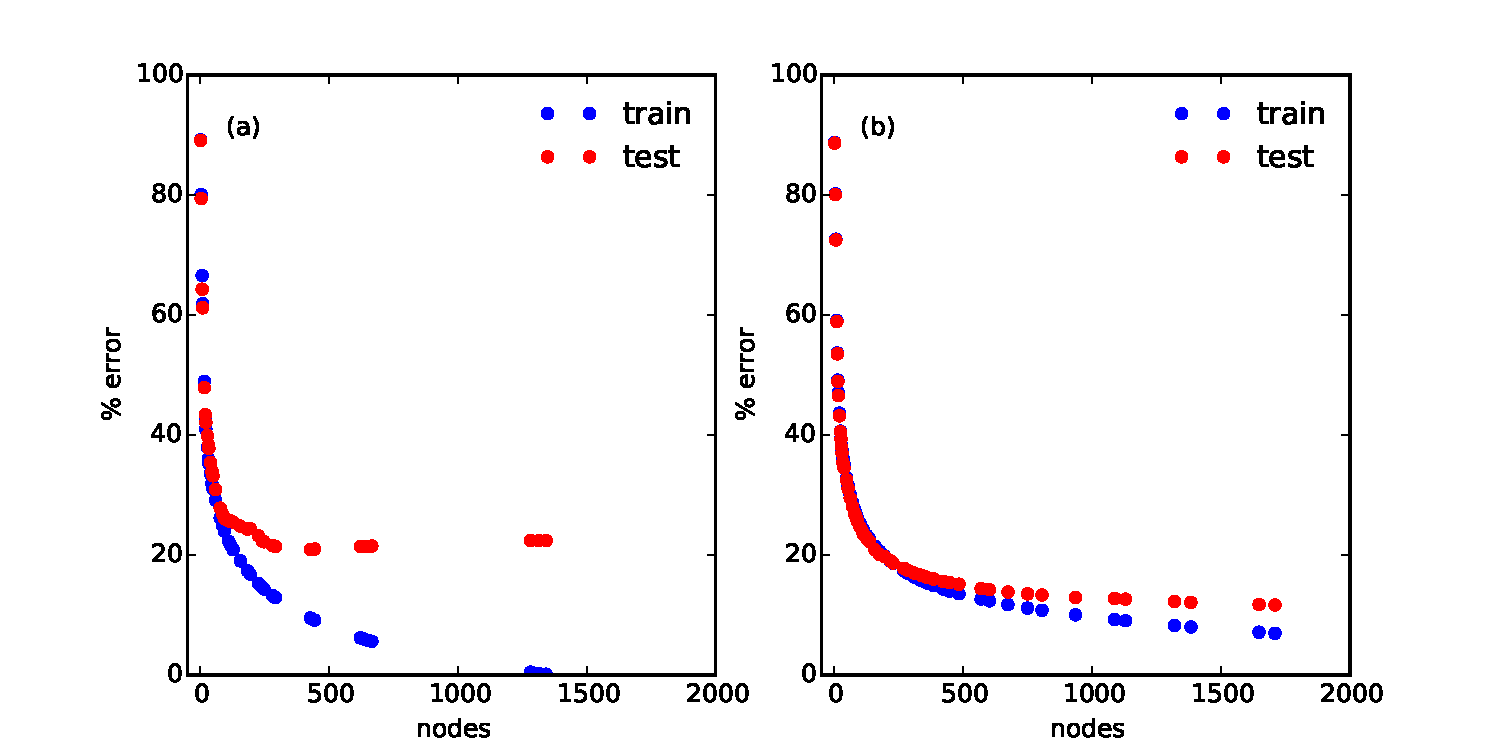
\includegraphics[width=5in]{../results/mnist/dtree/error_vs_nodes.pdf}
	\end{center}
	\caption{Misclassification rate of the decision tree algorithm increasing number of nodes. The size of the training data is (a) 6000, (b) 60000 training samples.\label{dtree2}}
\end{figure}
%%

Figures \ref{dtree1} and \ref{dtree2} suggest that optimum pruning point for a {\em single} decision tree algorithm would be around $\texttt{maxdepth}=15$ and $\texttt{complexityParameter}=10^{-4}$ resulting in trees with about 1000 nodes. 

{\bf Model improvement:} In the present experiments, a single decision tree trained on the entire dataset is able to achieve only about 12\% misclassification rate on the test set. This is consistent with the general observation that decision trees are prone to overfitting especially for datasets having a large number of closely spaced features such as in the MNIST dataset. The overfitting also suggests that ensembles of trees, either in the form of random forests or boosting, may perform better. 
%%
\subsection{Boosted tree ensembles}
Boosted decision trees have performed well on the MNIST dataset~\cite{kegl}. However the iterations needed to obtain these performances are prohibitively high for our computing resources. For example, the 1.26\% test error rate requires $T = 10^5$ iterations on the full MNIST dataset \cite{kegl}. In contrast, our training times were $\sim$5 minutes for 100 iterations on a 10\% sample of the data (6000 training examples). As a result, we seek to evaluate boosted tree ensembles differently.

We fix the sizes of the training and testing sets to 6000 and 1000 examples respectively. We then train a single large tree with {\tt maxrepth} = 30 and 400 nodes and a boosted ensemble with 200 base learners. Our boosting is performed using the AdaBoost.M1 algorithm in R's {\tt adabag} package. Finally we contrast the performance of these three learners.  

The base learner for this section is a decision tree of {\tt maxdepth} of 5 with 50 nodes. The training and test errors of the base learner are 31.45\% and 32.4\% respectively. While the base learner is clearly underfitting, it satisfies the criterion for being a weak learner.  

As evident from Fig~\ref{boost1}, boosting significantly improves performance of a single base learner. To get a comparable performance from a single tree, one needs a tree with over 400 nodes. Such large trees are susceptible to overfitting over unseen test data (although they don't in this particular instance). 

{\bf Model improvement:} Trees ensembles are preferable over single large trees because of better generalization. However, as the MNIST dataset illustrates, boosted trees are costly to train for high dimensional data. To improve our model here, clearly we need to increase the training data size and the number of boosting iterations. Both of these improvements are outside the range of our present computational resources for the present dataset. One option for model improvements for the present dataset might be to use random forest ensembles instead of boosted trees since the former tend to be more computationally feasible. 
%%
\begin{figure}[tbp]
	\begin{center}
	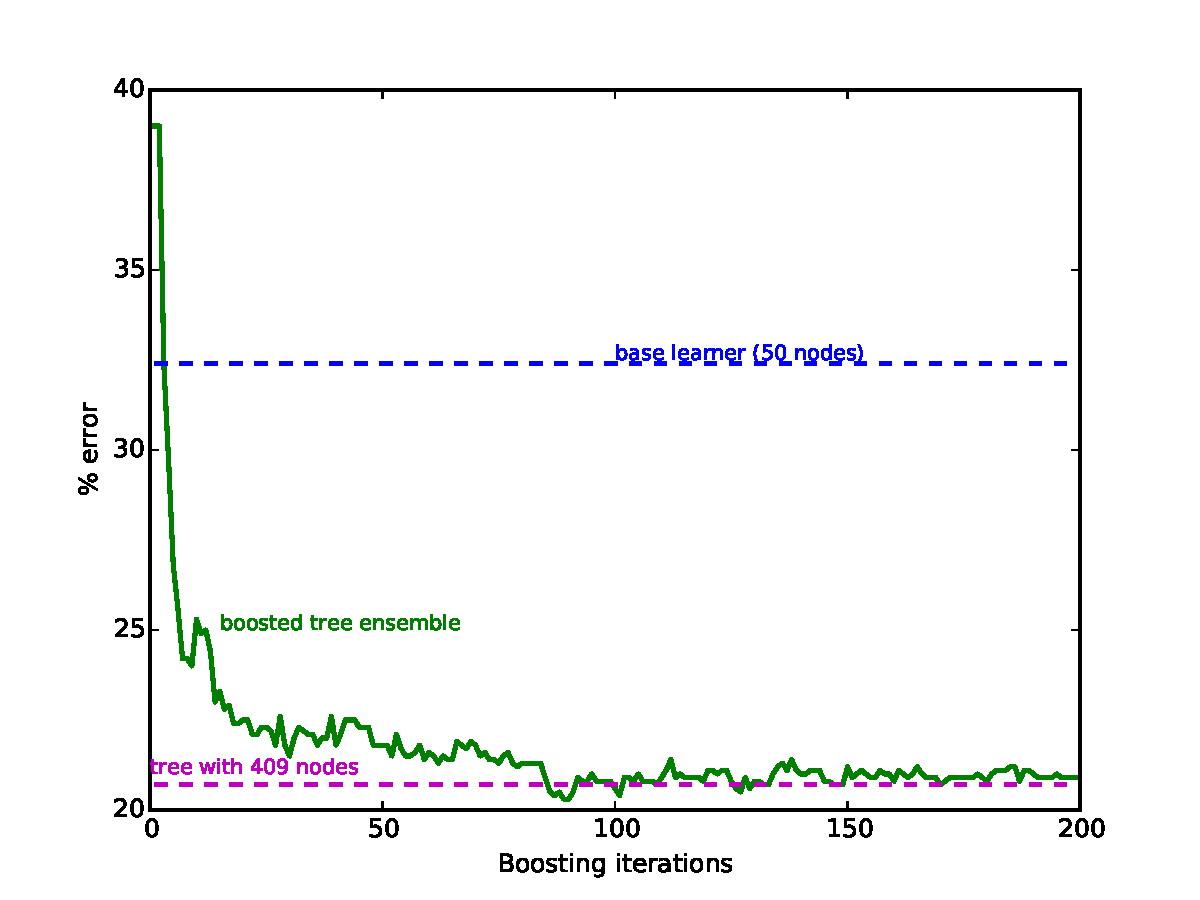
\includegraphics[width=3in]{../results/mnist/boosting/error_vs_boosting_iters.pdf}
	\end{center}
	\caption{Misclassification rate of the a single base learner with 50 nodes ({\color{blue} blue}), a boosted ensemble of base learners ({\color{green} green}), and a single learner with 409 nodes. ({\color{magenta} magenta}) \label{boost1}}
\end{figure}
%%

%
\subsection{Support vector machines (SVM)}
Support vector classifiers seek to find the optimum separating hyperplane while still minimizing the misclassified points. Mathematically, a (linear) SVM problem is expressed as:
\begin{align}
	\argmin_{w}\,\, \frac{1}{2}\|w\|^2 + C \sum_{i=1}^N\xi_i  \nonumber \\
	\text{subject to } \xi_i > 0 \text{ and } y_i(x_i^Tw) > 1-\xi_i \label{svmeq}
\end{align}
where $C$ is the `cost' parameter that determines the relative importance of the mis-classified points in computing the optimum hyperplane. To see this, note that making $C\to\infty$ will de-emphasize the minimization of `weights' and fit a complicated boundary to the training data. In contrast, making $C\to 0$ will tend to de-emphasize minimization of mis-classification cost. In other words, large values of $C$ tend to overfitting and small values of $C$ tend to underfit. The optimum value of $C$ is found from cross validation. 
%%
\begin{figure}[tbp]
	\begin{center}
	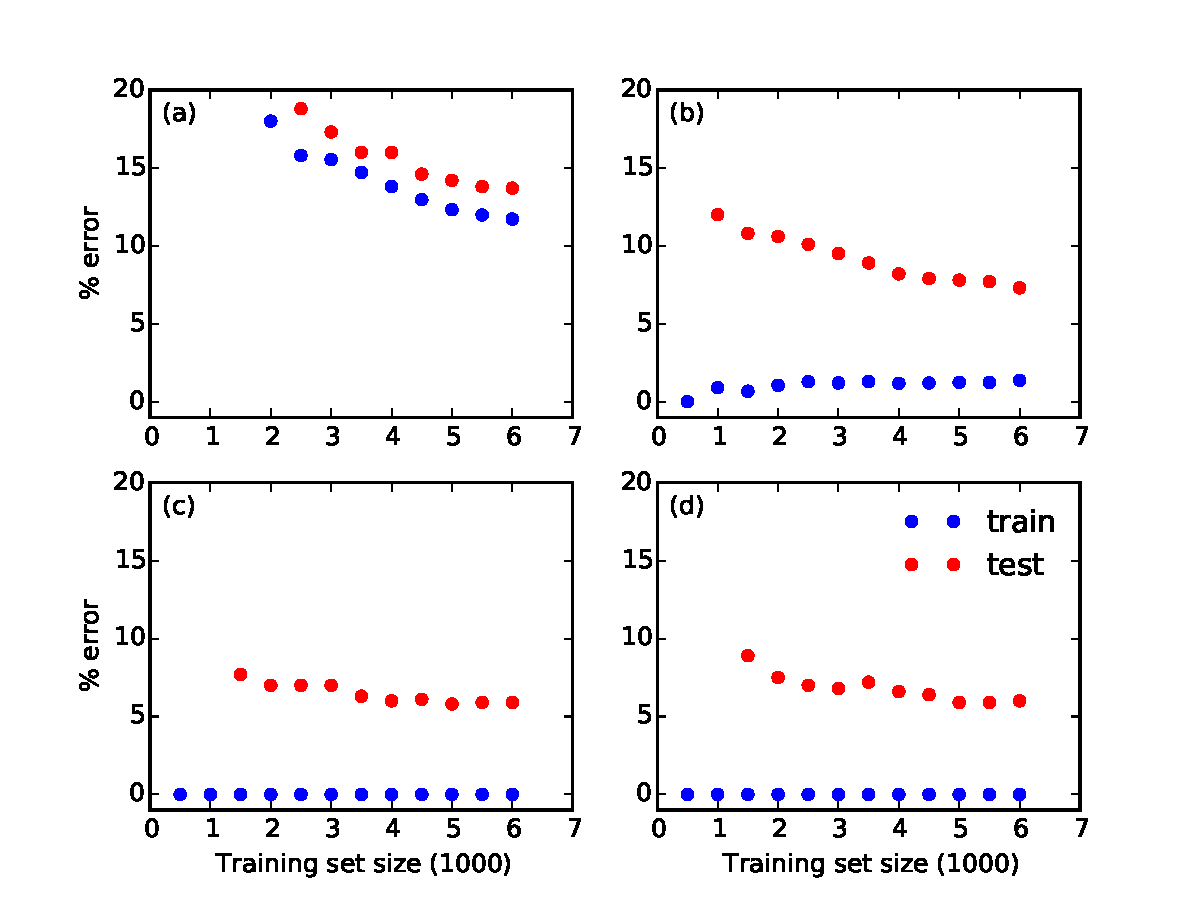
\includegraphics[width=4in]{../results/mnist/svm/error_vs_training_size.pdf}
	\end{center}
	\caption{Misclassification rate of the SVM algorithm with RBF kernel as a function of training size for different values of the cost parameter $C$. (a) $C=0.1$, (b) $C=1$ (c) $C=10$ (d) $C=10^5$.\label{svm1}}
\end{figure}
%%

Below we study the performance of SVM models trained on MNIST data using radial basis function (RBF) and polynomial kernels. 

\subsubsection{SVM with radial basis functions (RBF) kernel}
While packages in R allow us to perform automatic cross-validation, it is instructive to visualize evolution of training and test errors with training data size for various values of $C$. Figure~\ref{svm1} plots this error evolution for $C = 0.1, 1.0, 10.0 \text{ and } 10^5$. 

The training and the testing errors show a clear trend until $C\leq10$. The model is less sensitive to $C$ for $C\gtrsim10$. An inspection of \myeqno{svmeq} reveals that this behavior is expected at some threshold value of $C$. After this threshold, the `weights' term is fully de-emphasized giving an essentially unregularized model. Yet there is no evidence of overfitting. This is possibly because there is still enough training data as apparent from the decrease in the test error with increasing data. 
%%
\subsubsection{Comparisons of SVM with polynomial and RBF kernels}
%%
\begin{figure}[tbp]
	\begin{center}
	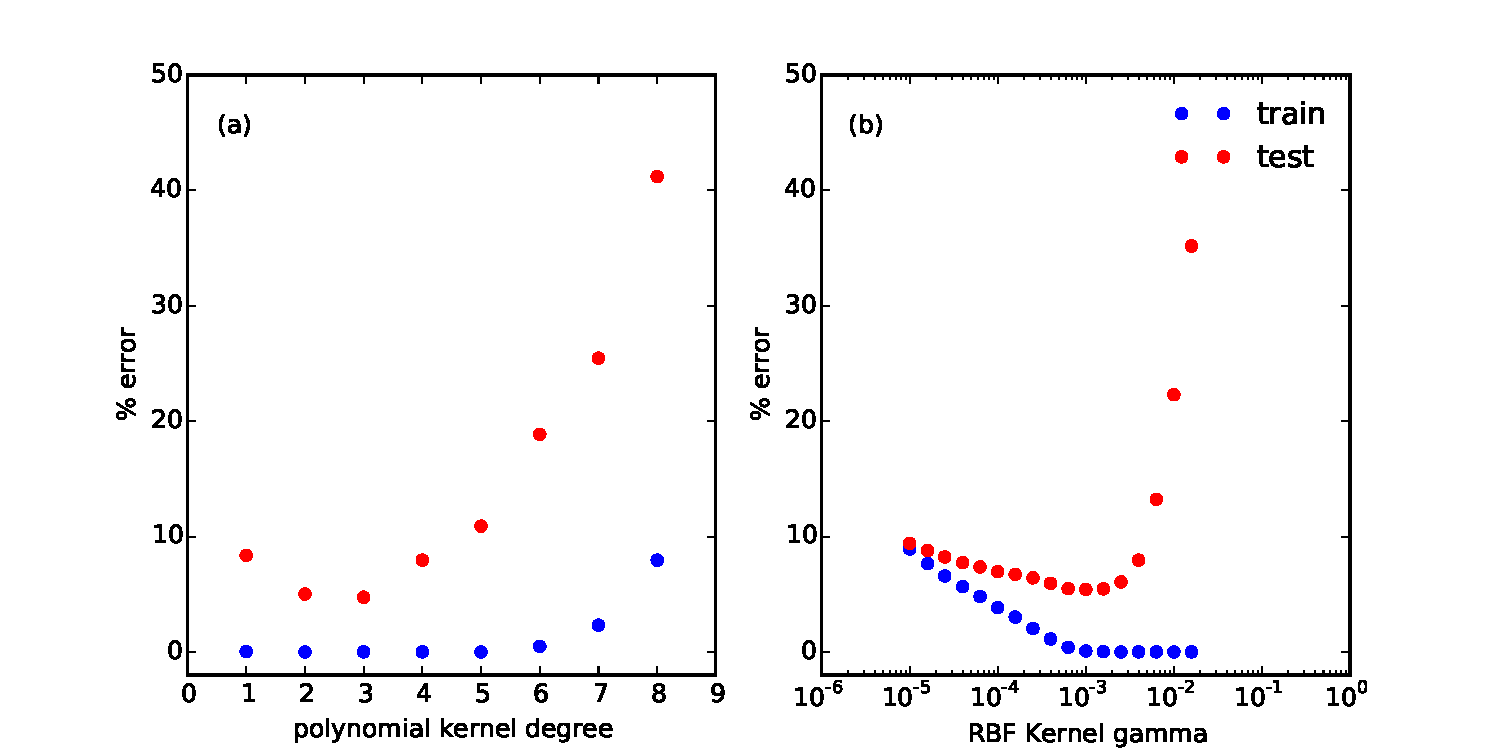
\includegraphics[width=4in]{../results/mnist/svm/error_vs_complexity.pdf}
	\end{center}
	\caption{Misclassification rate of the SVM algorithm with (a) polynomial kernel as a function of its degree and (b) RBF kernel as a function of parameter $\gamma$. For both cases, the model is trained on 6000 samples and the `cost' parameter is fixed at $C=10$. \label{svm2}}
\end{figure}
%%
For this study we fix the `cost' parameter to $C=10$. The complexity of the polynomial kernel is tuned by the degree of the polynomial. We study the training and the test error as a function of the kernel degree. For the RBF kernel, the complexity is controlled by the $\gamma$ parameter in the kernel ($K(x,y) \equiv e^{-\gamma \|x-y\|^2}$). The model is trained on 6000 samples and tested on all 10000 samples. 

For the polynomial kernel, the test error is minimum ( = 4.74\%) for a degree 3 polynomial kernel. The test error increases rapidly for higher degree polynomials due to overfitting. For the RBF kernel, there is a clear evidence of a transition from underfit to optimal fit to overfit as the width parameter $\gamma$ is varied. The optimum point for RBF kernel gives a minimum error of 5.42 \% and was located using cross validation. $\gamma$ was then varied about this point to study the effect of this variation on training and testing errors.

As a final test, we trained the optimized SVMs with RBF ($\gamma = 0.001$) and polynomial (degree = 3) kernels on the full MNIST dataset and obtained the performance reported in Table~\ref{tab1}.

{\bf Model improvement:} The RBF and Polynomial SVMs are able to achieve respectively 2.2\% and 2.64\% test error rates on the full MNIST dataset. The state of the art reported by the LeCun et al for SVMs is 1.4\%~\cite{mnist}. The reason for this difference is as follows. Our model hyperparameters ($C$, $\gamma$ and degree) were obtained from cross-validation on a 10\% sample of the full data. Therefore, one obvious way to improve the model performance is to determine the hypermarameters by cross validation on the {\em full} MNIST dataset. Additionally it might be worthwhile to explore effect of data normalization: centering + unit variance. 
%%
\begin{table}[tbp]
	\caption{{\bf SVM best results:} Training and test errors of the optimized SVM models with RBF and polynomial kernels on the full MNIST dataset (training set = 60,000, test set = 10,000 instances).\label{tab1}}
	\centering
    \begin{tabular}{c|c|c|c}
         \hline
            	{\bf Kernel}&{\bf training error} & {\bf test error} & {\bf training time}\\ \hline \hline
            	RBF, $C=10, \gamma=0.001$&0.19\%&2.20\% & 30 minutes\\	
            	Polynomial, $C=10$, degree = 3&0.77\%&2.64\% & 30 minutes\\ \hline
    \end{tabular}
\end{table}
%%
\subsection{Neural networks}
Our neural net architecture of choice is a feed-forward neural networks with a single hidden layer. With this choice, the only free parameter is the number of units in the hidden layer. The number of hidden units used for the MNIST dataset in the literature has varied between 300 and 1000~\cite{mnist}. We found that training even a single-hidden layer feed forward NN with $>30$ hidden units takes roughly 10 minutes on our laptop and prohibits exhaustive experimentation. We therefore study the behavior of the algorithm up to a modest number of hidden layer nodes ($\sim 50$) and try to infer any visible trends. 

Our neural net is implemented using the {\tt nnet} library in R. This library is capable of modeling feed-forward neural networks with a single
hidden layer and is a good choice given our computational resources. To study the neural network, we varied the number of hidden layer units between 5 and 30 and the sample size drawn from the training set between 600 and 60000 (i.e. 1\% to 100\% of the MNIST dataset). The test set size was 10000 for all the observations.  
%%
\begin{figure}[!tbp]
	\begin{center}
	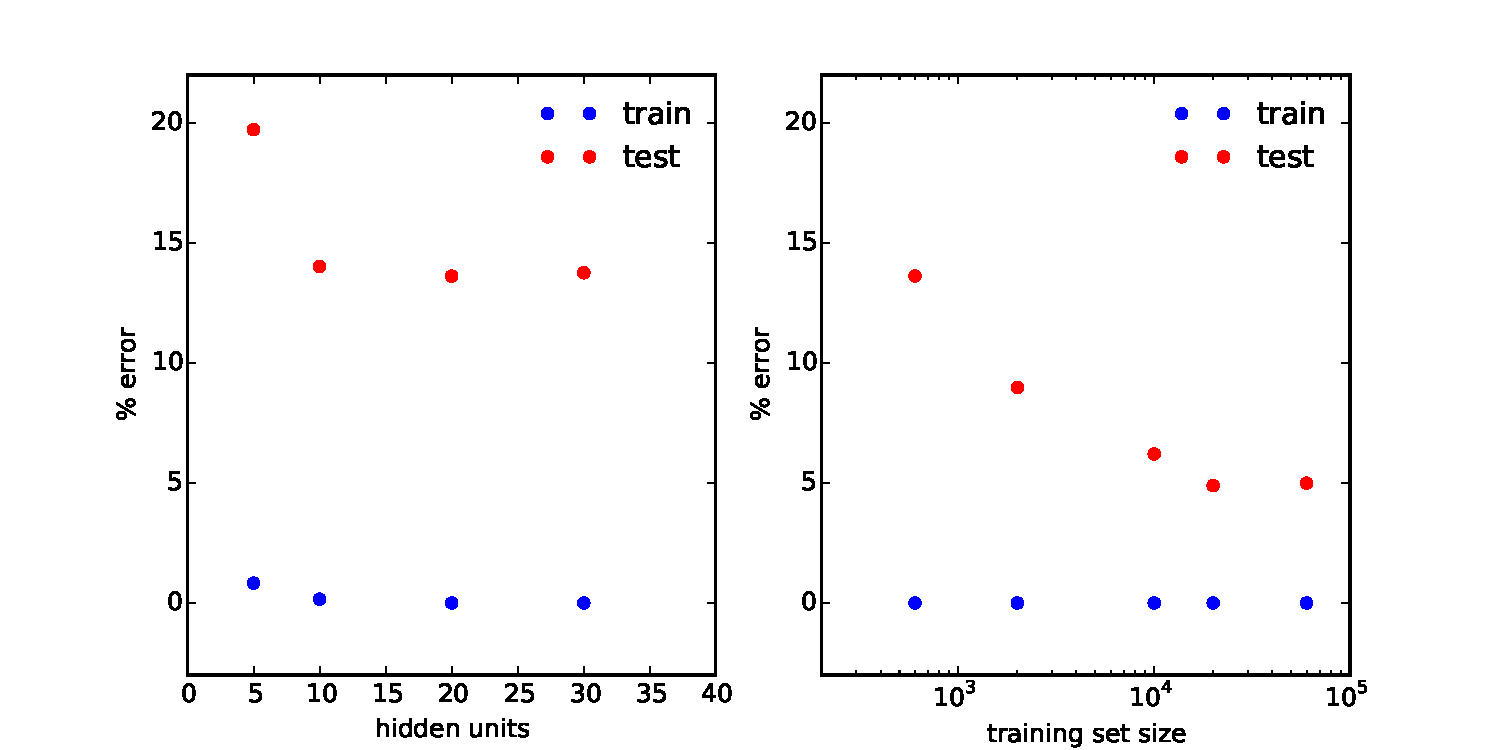
\includegraphics[width=4in]{../results/mnist/nnet/error_vs_hidden_units_and_training_size.pdf}
	\end{center}
	\caption{Misclassification rate of the one-hidden-layer feed-forward neural network as a function of (a) number of hidden units and (b) training set size \label{nnet1}}
\end{figure}
%%

The evolution of the training and test errors are plotted in Fig.~\ref{nnet1}. The test error first decreases with number of hidden units ($N_h$) and saturates between $10 < N_h < 20$. The test error, however drops from 14.0\% to 4.9\% as the size of the training set is increased from 600 to 20000 samples and plateaus thereafter, indicating an optimal fit. For these parameters, the network training time also increased from 414 seconds to about 1800 seconds (30 minutes). As a final test, we trained the neural network with 50 hidden units on the entire MNIST training data and obtained the results displayed in Table~\ref{tab2}.  
%%
\begin{table}[tbp]
	\caption{{\bf Neural network best results:} Training and test errors for a 50 unit, one-hidden-layer feed-forward neural network (training set = 60,000, test set = 10,000 instances).\label{tab2}}
	\centering
    \begin{tabular}{c|c|c|c}
         \hline
            	{\bf Neural network}&{\bf training error} & {\bf test error} & {\bf training time}\\ \hline \hline
            	1-hidden layer, 50 hidden units&0.00166\%&2.57\% & 3.5 hours\\ \hline
    \end{tabular}
\end{table}
%%

{\bf Model improvement:} The values reported by LeCun for a one-hidden-layer net with 300 hidden units is 4.7\%. This compares favorably to our value of 4.9\% obtained with just 20 hidden units. With 50 hidden units the test error drops to 2.57\% and performs better than some reported models which employ pre-processing and up to 1000 hidden units\cite{mnist}. It seems that we've pushed the single-hidden-layer neural network to its limit (without using any pre-processing). As suggested by the MNIST website~\cite{mnist} further improvements will need us to either use multi-layer networks or use the domain knowledge of the images to perform preprocessing operations such as de-skewing and elastic distortions. 
%%
%%
\section{Supervised learning algorithms on the Ionosphere data}
We now turn to applying various learning algorithms to our second dataset, the ionosphere data. The algorithms perform mostly similarly to how they did on the MNIST data. Our descriptions will therefore be shorter compared to the previous section; the differences, when they arise, will be pointed out. 
\subsection{k nearest neighbors (KNN)}
As mentioned previously, accurate predictions using KNN requires large amounts of data, especially as the number of attributes increase. Here  we have 150 data points to determine nearest neighbors in 34 dimensions. We trained on the entire training data and varied nearest neighbors from 1 to 11. As depicted in Fig~\ref{knnion1}, $k=3$ achieves the lowest error rate of 11.44\%. As we increase $k$, the model suffers from under-fitting as evidenced by increase in both training and test errors. 
%%
\begin{figure}[!tbp]
	\begin{center}
	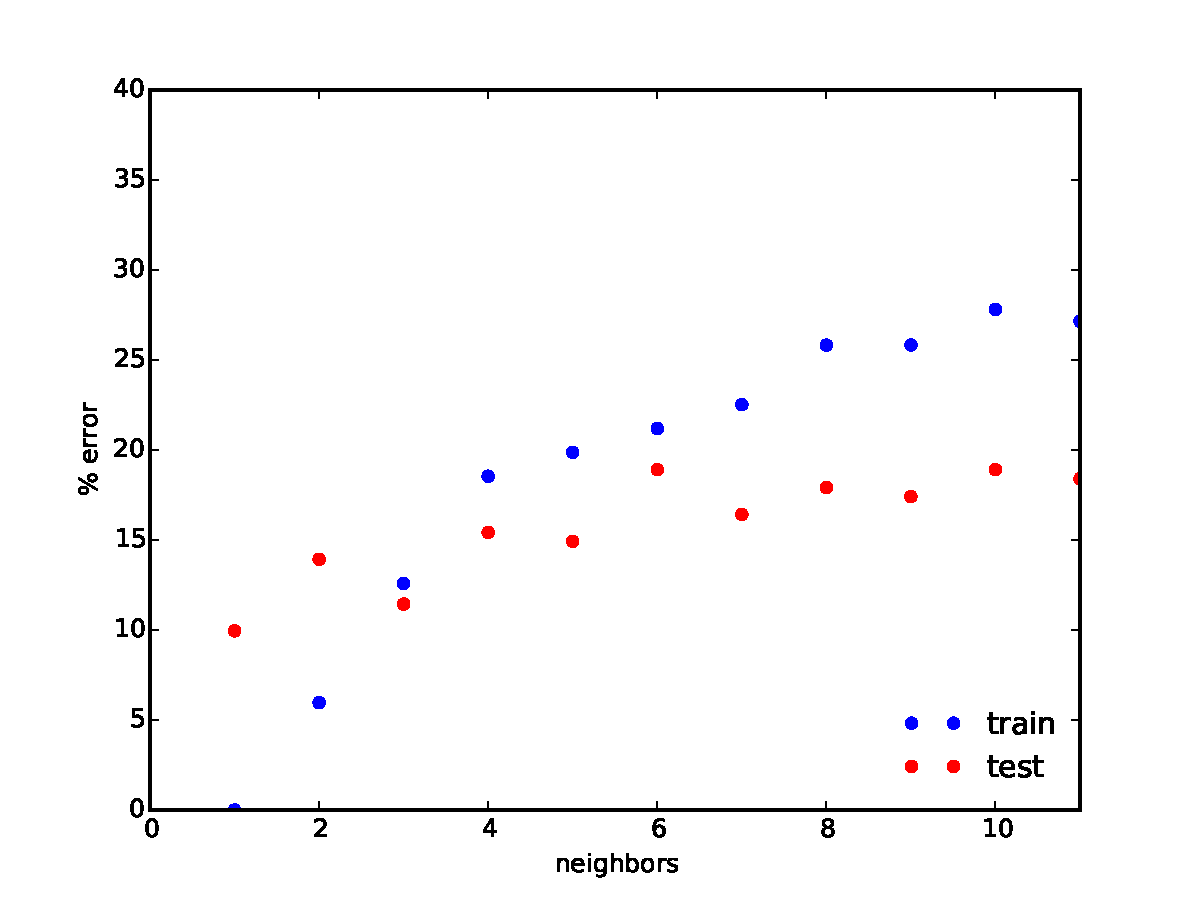
\includegraphics[width=2.5in]{../results/ionosphere/knn/error_vs_nbrs.pdf}
	\end{center}
	\caption{Misclassification rate of the KNN algorithm on the ionosphere training and test data for different nearest neighbors\label{knnion1}}
\end{figure}
%%

{\bf Model improvement:} Although use here for comparative purposes, KNN is not a good model for this dataset because of the small amount of available training data relative to number of dimensions. As with MNIST, one could explore reducing dimensionality of the problem to get rid of correlated features and make the KNN model work better. One could also perform a different train:test split of the input data. But that is cheating and is likely not possible in real life :)
%%
\subsection{Decision trees}
This is an ideal problem for decision trees as we have a moderate number of discretely valued input features. As in the case of MNIST we determined the optimum pruning point by varying the tree depth from 2 (stump) to 30 (max allowed by {\tt rpart} package in R). Fig.~\ref{dtreeion1} shows the variation of the training and testing errors for trees of increasing complexity (depth). From the figure, a decision tree with depth of 2 achieves an 10.1\% error rate an appears to be an optimum pruning point.   
%%
\begin{figure}[!tbp]
	\begin{center}
	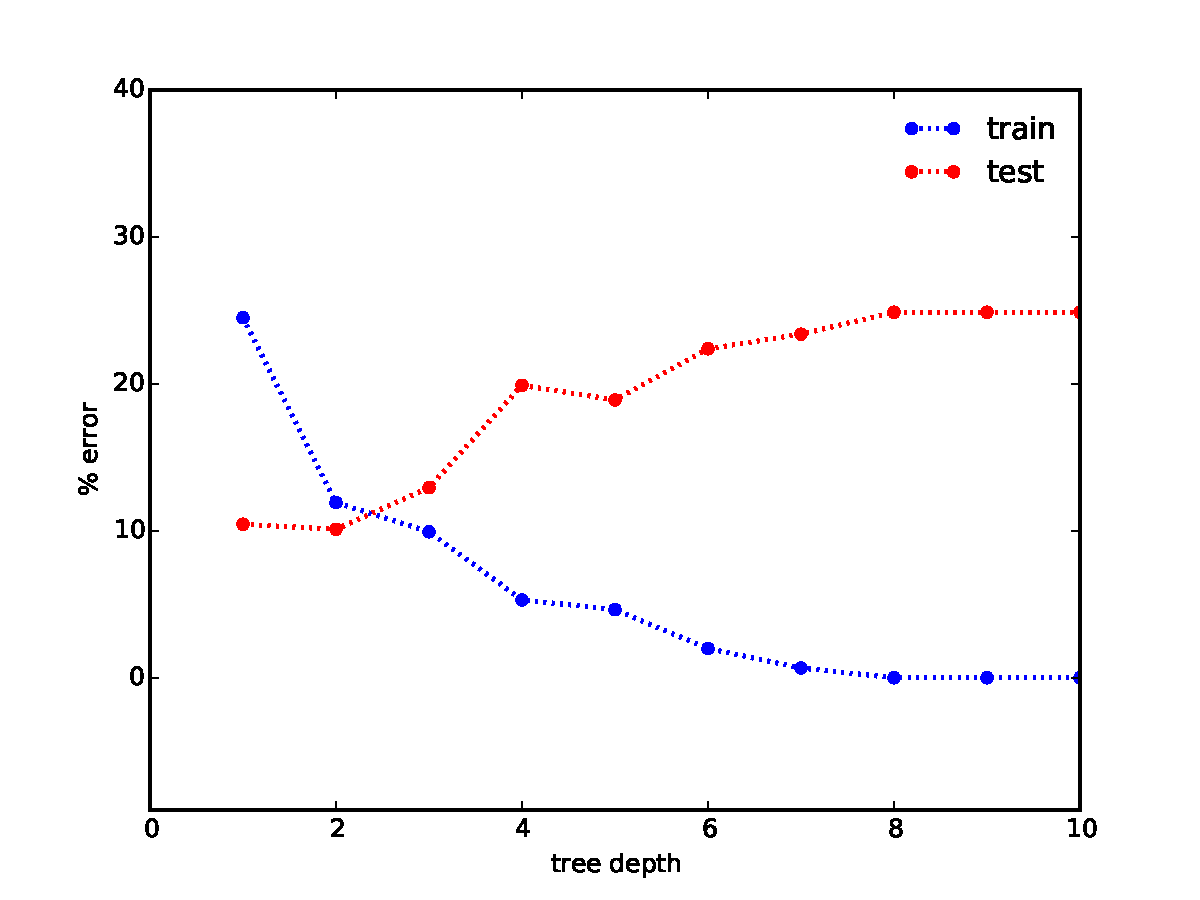
\includegraphics[width=2.5in]{../results/ionosphere/dtree/train_test_error_vs_depth.pdf}
	\end{center}
	\caption{Misclassification rate of the single decision tree algorithm for increasing tree depth. \label{dtreeion1}}
\end{figure}
%%

{\bf Model improvement:} Achieving optimum performance at {\tt maxdepth} = 2 indicates that a single feature is dominating the information gain in the data. It also appears that at {\tt maxdepth} = 2 the training error is still 11\% which indicates underfitting. As we increase the tree depth, the training error goes down, but and the test error goes up. Both these aspects strongly suggest that gathering more data is likely to improve model performance. It might also be worthwhile to see if tree ensembles lead to better generalization. However, if the underlying issue is the lack of adequate data, then boosting is unlikely to produce significant benefits.  
%%
\subsection{Boosted tree ensembles}
We construct boosted ensembles of weak trees using the AdaBoost.M1 algorithm provided by the {\tt adabag} package in R. Fig.~\ref{boostion1} shows the results of fitting a boosted tree to the data. The base learner here is a stump achieves about 10.1\% error rate. We applied 1000 boosting iterations to this base learner which brought its error rate down to about 7.96\%. For this dataset, boosting provides a modest 2\% improvement over individual trees.
%%
\begin{figure}[!tbp]
	\begin{center}
	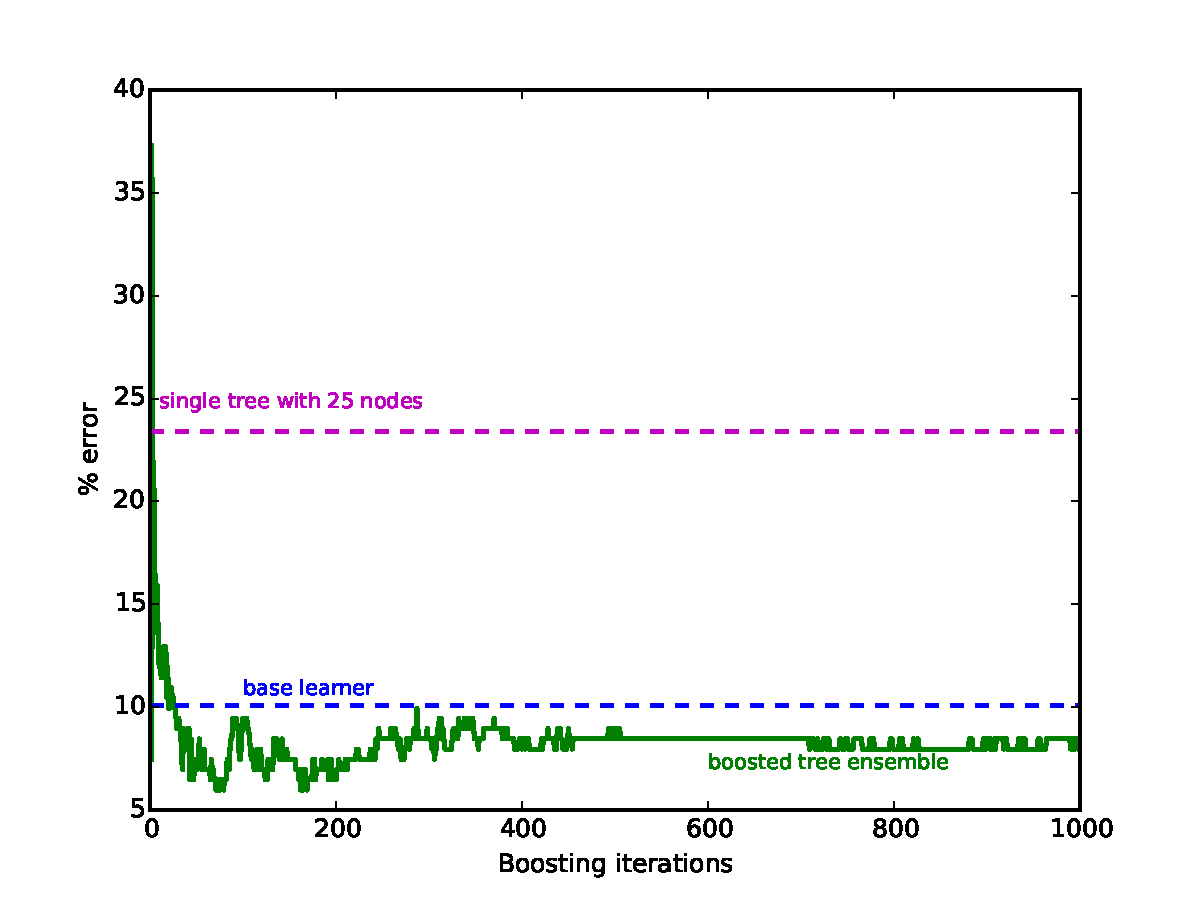
\includegraphics[width=2.5in]{../results/ionosphere/boosting/error_vs_boosting_iterations.pdf}
	\end{center}
	\caption{Misclassification rate of boosted tree ensemble with number of boosting iterations (base learners). \label{boostion1}}
\end{figure}
%%

{\bf Model improvement:} It appears that the accuracy has plateaued after 1000 iterations. As seen in the previous section,  the issue in this case appears to be inadequate amount of data. This is perhaps the reason why we saw boosting provide only modest gains. As such, the recommendation in the previous section (`gather more data') still applies. 
%%
\subsection{Support vector machines (SVM)}
SVMs were implemented using the {\tt e1071} package in R. Fig.~\ref{svmion1} shows the variation of training and test error for variation in the `cost' parameter (which controls regularization) and the kernel width $\gamma$. The results show that the optimum point is obtained at $\text{cost }=71$ and $\gamma = 10^{-3}$ leading to a test error of 6.5\%. 
%%
\begin{figure}[!tbp]
	\begin{center}
	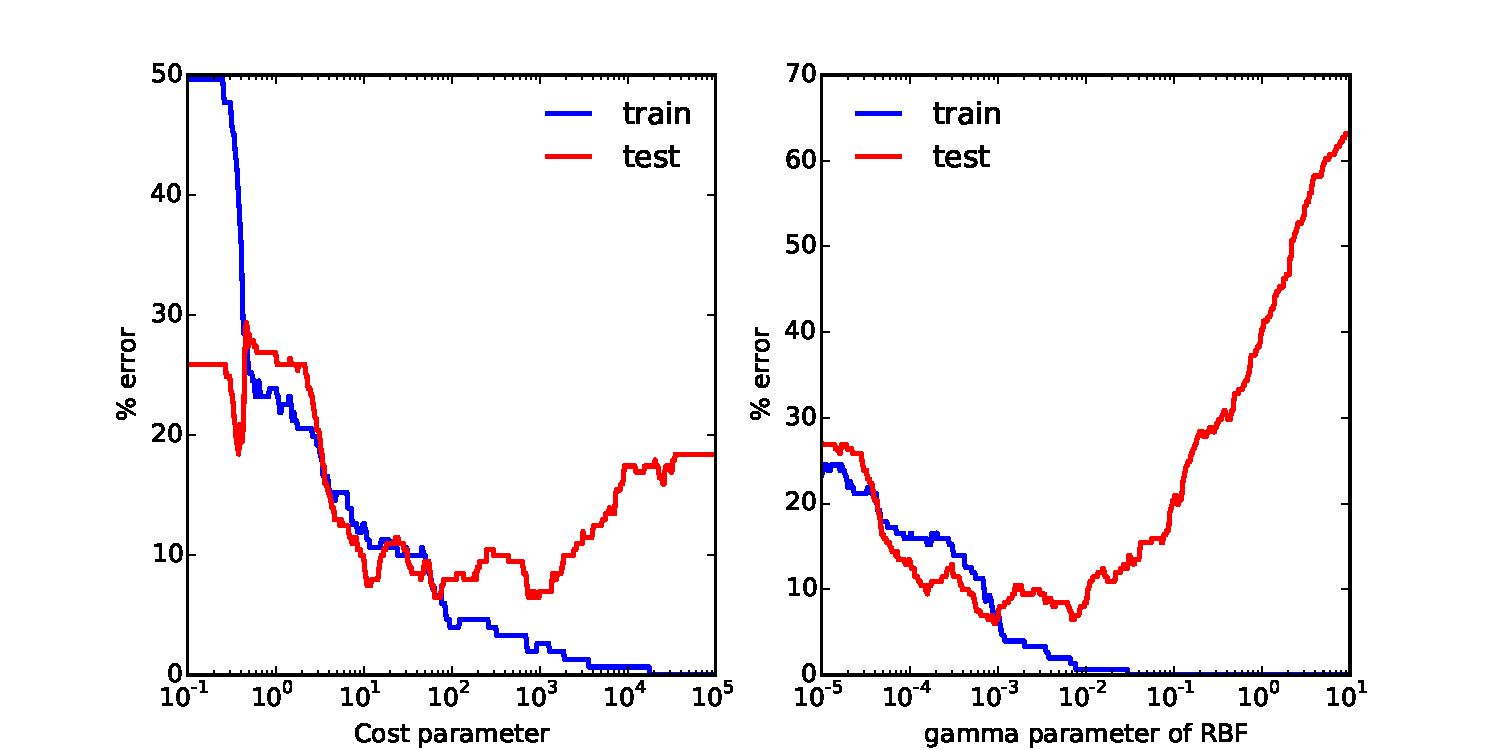
\includegraphics[width=4in]{../results/ionosphere/svm/error_vs_cost_gamma.pdf}
	\end{center}
	\caption{Misclassification rate of the SVM algorithm under variation of (a) the cost (regularization) parameter for $\gamma=10^{-3}$ and (b) the kernel width $\gamma$ for $\text{cost }=70 $. \label{svmion1}}
\end{figure}
%%

{\bf Model improvement: } The accuracy numbers obtained by SVMs, $\sim 93.5\%$ are comparable to the ones reported in the literature (using other algorithms) \cite{ionosphere}. It also seems that the optimum point is obtained where the model is still underfitting. This calls, as before, for more training data. 
%%
\subsection{Neural networks}
The final model we train on the data is a one-hidden-layer, feed-forward neural network with varying number of hidden units. As before we used R's {\tt nnet} package. With neural nets we're able to achieve 6.6\% test error rate for 100 hidden units (Fig.~\ref{nnetion1}).

The small size of the training data allowed us to reach network sizes up to 100 hidden units at which point the error plateaued.
%%
\begin{figure}[!tbp]
	\begin{center}
	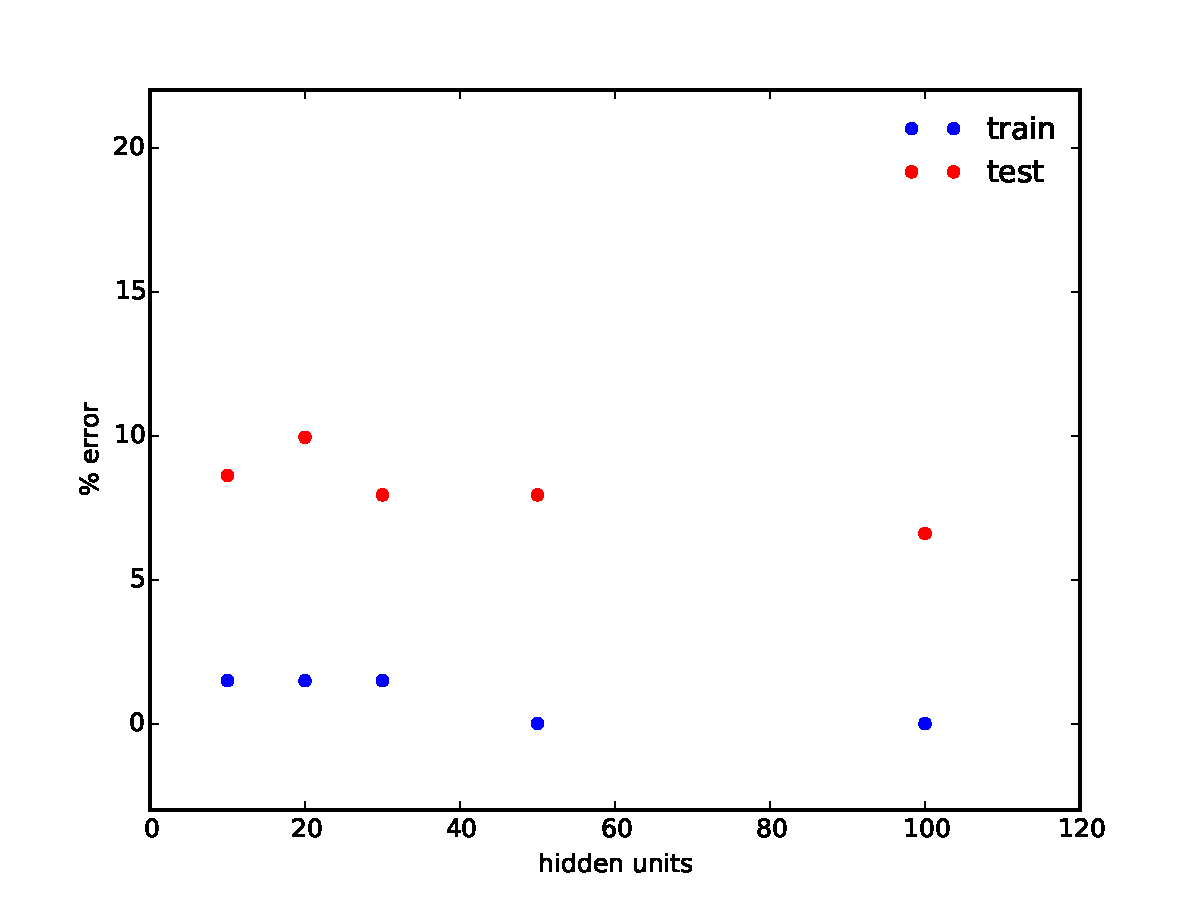
\includegraphics[width=2.5in]{../results/ionosphere/nnet/error_vs_hidden_units.pdf}
	\end{center}
	\caption{Misclassification rate of one-hidden-layer feed-forward neural networks with different number of hidden units. \label{nnetion1}}
\end{figure}
%%

{\bf Model improvement: } Figure~\ref{nnet1} indicates how crucial the size of the training data is for neural net performance. So even for neural nets, improving performance will depend on getting more training data for this problem. In addition, it might be worthwhile to explore data normalization to see if it results in extra performance gains. 
%%
\section{Model comparison}
Finally we summarize our studies by collecting in one place the performance of our implementation and comparing them with the numbers reported in the literature for these datasets. The primary limiting factor for our algorithms has been the training time or, equivalently, the computational resources. Also in the case of ionosphere data, the train/test split is not known for to enable us to make fair comparisons (we cannot access the original papers). 
\begin{table}[tbp]
	\caption{ Comparison of different algorithms. The reported numbers for MNIST can be found in \cite{mnist} and those for the ionosphere study can be found in \cite{ionosphere}\label{tab3}}
	\centering
    \begin{tabular}{p{2cm}|p{2.75cm}|p{1.2cm}|p{1cm}|p{2.75cm}}
         \hline
            	{\bf Dataset}&{\bf Algorithm} & {\bf Training set size} & {\bf Test error} & {\bf Best \,\,reported}\\ \hline \hline
		MNIST & KNN, $k=10$ & 6000 & 6.6\% & 5.0\% using full data \\ \hline
		MNIST & single decision tree & 60000 & 12.0\% & unknown \\ \hline
		MNIST & boosted trees, 200 iters & 6000 & 20\% & 1.26\% with $10^5$ iterations, using full data \\  \hline
		MNIST & SVM, $C=10, \gamma=0.001$ & 60000 & 2.2\% & 1.4\% \\ \hline 
		MNIST & Neural net, 1 hidden layer, 50 hidden units & 60000 & 2.57\% & 4.7\% \\ \hline
		Ionosphere & KNN, $k=3$ & 150 & 10\% & 9\% (train/test split unknown) \\ \hline
		Ionosphere & single decision tree & 150 & 10\% & unknown \\ \hline
		Ionosphere & boosted trees, 1000 iters & 150 & 7.96\% & unknown \\ \hline
		Ionosphere & SVM $C=71, \gamma=0.001$ & 150 & 6.6\% & unknown \\ \hline
		Ionosphere & Neural net, 1 hidden layer, 100 hidden units & 150 & 6.5\% & 4.5\% (train/test split unknown) \\ \hline 
    \end{tabular}
\end{table}
%%
\end{document}













